\documentclass{article}
\usepackage{../fasy-hw}
\usepackage{algpseudocode}

%% UPDATE these variables:
\renewcommand{\hwnum}{6}
\title{Discrete Structures, Homework \hwnum}
\author{Peyton Meeks}
\collab{n/a}
\date{due: 6 April 2021}

\begin{document}

\maketitle

This homework assignment should be
submitted as a single PDF file both to D2L and to Gradescope.

General homework expectations:
\begin{itemize}
    \item Homework should be typeset using LaTex.
    \item Answers should be in complete sentences and proofread.
    \item You will not plagiarize, nor will you share your written solutions
        with classmates.
    \item List collaborators at the start of each question using the \texttt{collab} command.
    \item Put your answers where the \texttt{todo} command currently is (and
        remove the \texttt{todo}, but not the word \texttt{Answer}).
\end{itemize}


% ============================================
% ============================================
\collab{n/a} \nextprob{Applications}
% ============================================
% ============================================

The topics in this class are mathematical in nature, but have strong ties to
computer science: either for understanding how computers work, why alogithms are
correct, or for how to convert real-world data into things that can be analyzed
using a computer.  Explain how each of the following tie to computer science or
data science:

\begin{enumerate}

    \item Tree (be sure that your answer needs a tree, and not a general graph)

        \paragraph{Answer}

       A Tree can be used with regards to computer science when we think about algorithms, specifically priority queues. Priority queues are a type of sorting algorithm where one element that is not entered first can have a higher desired value, priority, that an element entered before it, and therefore be moved to the top of the queue.

    \item Directed Graph

        \paragraph{Answer}

       Directed Graphs are graphs in which an edge points from one vertex to another, and these are very useful in computer and data science. For example a directed graph could be used to analyze the data flow of a network of computers to see where optimization could be implemented. 
    \item Equivalence Classes

        \paragraph{Answer}

        Eqivalence classes are important to computer science becuase of the value that they provide in being able to relate what appear to be unrelated, or difficult to define items to something much easier to define. An example of this is the equivalence class that relates the ascii code for which a computer processes and stores data to the alphabet that we are use to. Each letter, number, and symbol has an ascii code which is stored in your computers database and accessed with conversion algorithms so that we do not have to memorize the extremply complex code to use a computer for everyday tasks.

<<<<<<< HEAD
    \item Distance Metrics

        \paragraph{Answer}

        A distance metric is the distance that defines the seperation of a set of points. This is used in computer science to help optimize networks or algorithms to produce faster and more accurate results. One example would be a search algorithm designed to measure the distance between search results and return the result with the shortest distance, closest result, to the input.

=======
>>>>>>> 6bd2741a5a93eaad31d8ff1277dd11d1f0b178a2
    \item Injective Function

        \paragraph{Answer}

        An injective function is useful for computer and data scientists to find relations, or lack there of of functions. Since an injective function is a one to one function, each point in the domain must point to a different point in the co-domain. This is useful for many algorithms so that an input can be proven to have a specific output.


\end{enumerate}


% ============================================
% ============================================
\collab{n/a} \nextprob{Distance Functions}
% ============================================
% ============================================

Suppose you maintain a database of cocktail recipes.  You want to write a
application that asks a user for their favorite cocktail and returns a cocktail
that they might like.  To do so, you define the distance between two cocktails
to be the symmetric distance between their ingredient lists.  Then, for the
input cocktail, you compute the distance to every cocktail in your database and
return one of the cocktails that minimizes this distance.

\begin{enumerate}

    \item Prove that this distance is a metric. (Note: first, formally write out
        what the distance function is, including the domain and codomain).

        \paragraph{Answer}

        Let the domain $X$ be the set containing all of the ingredients of the inputed cocktail and the co-domain $Y$ be the set, database, containing all subsets $C$ such that $C$ is a list of a cocktail's different ingredients. Then the distance function $F$ can be described as $F: X \rightarrow C \rightarrow Y$. Where for any ingredients $x,y,z \in X$, all ingredients are of equal value such that $x \gets y$ and $y \gets x$ also, $F(x,y)= F(y,x)=0$. This means that $0=F(x,x) \leq F(x,y) +F(y,x) = F(x,y) + F(x,y)=2F(x,y)$. Since the three axioms of a metric are satisfied, then the distance is a metric.\footnote{“Metric (Mathematics).” Wikipedia, Wikimedia Foundation, 27 Mar. 2021, \url{en.wikipedia.org/wiki/Metric_(mathematics)}.}

    \item Is this a good distance to use for your application?  Why or why not?

        \paragraph{Answer}

       This is a good distance to use for the application because if an inputed cocktail's ingredient list has matches with one of the cocktail's ingredient lists in the database, this will return a distance of 0. This means that the overall distance will be decrease allowing for the matching of more similar cocktails to that of the one inputed.

\end{enumerate}


% ============================================
% ============================================
\collab{n/a} \nextprob{Loop Invariant}
% ============================================
% ============================================

Recall that a loop invariant is used to prove that a loop is correct (which in
turn helps to prove that an algorithm is correct).

\begin{enumerate}

    \item Write pseudocode that uses a while loop to find the second largest
        element in an unsorted array.  The input to your algorithm should be an
        unsorted array $A$ of real values.  The psuedocode should use the
        variable name \textsc{curguess} to store the current guess of the second
        largest value, and \textsc{curmax} to store the current max of $A$.

        \paragraph{Answer}

        \begin{algorithmic}
			\State float curmax=$A[0]$, curguess=null, 
			\State int $i=0$
			\State Find second largest real number in array $A$
				\While {$i$ != $size of A$}
					\If {$A[i]>=curmax$}
						\State $curguess=curmax$
						\State $curmax =A[i]$
						\State $i++$
					\EndIf
					\If {$A[i]>curguess$ and  $A[i] != curmax$}
						\State $curguess=A[i]$
						\State $i++$
					\EndIf
				\EndWhile \State
				\Return $curguess$
				
		\end{algorithmic}



    \item What is the postcondition of the loop? (Call this statement $Q$).

        \paragraph{Answer}

        \textsc{return(curguess), curguess=}second largest value of $A$.

    \item What is the precondition of the loop? (Call this statement $P$).

        \paragraph{Answer}

        $A$ is an inputed array of unsorted real numbers, \textsc{i=0, curmax=A[0], curguess=null}.

    \item What is the loop guard of the loop? (Call this statement $G$).

        \paragraph{Answer}

        $i \neq size of A$

    \item Prove that the loop invariant is when entering the $i^\text{th}$
        iteration of the loop is, ``the variable \textsc{curguess} stores
        the second
        largest value of $A[1,2, \ldots, i]$,
        and \textsc{curmax} stores the largest value of $A[1,2,\ldots, i]$.

        \paragraph{Answer}

        Let the loop invariant $I(n)$ be $i=n$, \textsc{curguess}=$A[n-1]$ for $n>0$ else $null$, and \textsc{curmax}=$A[n]$. Then the Basis Property $I(0)$ would be $i=0$, \textsc{curguess = $null$, curmax = $A[0]$}, which is true before the first iteration of the loop. Now using the inductive property, suppose k is a nonnegative integer such that $k+1$ is within the bounds of the array and $G I(k)$ is true before an iteration of the loop. Then before the next iteration of the loop  \textsc{curguess=$A[k-1]$, curmax=$A[k]$} and $i=k$. Since the guard $G$ is passed the algorithm enters the while loop. If $A[k] > curmax$ is true then, \textsc{curguess = $curmax_{old} = A[k]$, $curmax_{new} = A[k+1]$} and $i=k+1$. Hence after iterating the loop $I(k+1)$ is true for the first If statement. If $A[k]> curguess and A[k] \neq curmax$ then, after iterating through the loop, \textsc{$curguess_{new} = A[k]$, $curmax_{new}=curmax_{old}=A[k-1]$} and $i=k+1$. Hence after iterating this loop $I(k+1)$ is true for the second IF statement. Therefore since both IF statments are true after an iteration of the loop, The while loop is true and \textsc{curguess, curmax} will show the second highest value and the max value respectively.

\end{enumerate}



% ============================================
% ============================================
\collab{n/a} \nextprob{Four Colors Suffice}
% ============================================
% ============================================

Read Chapters $9$ and $10$ of \emph{Four Colors Suffice}.

\begin{enumerate}

    \item What is a \emph{reducible configuration}?

        \paragraph{Answer}
		
	   A reducible configuration is a arrangement of countries that cannot be used as a minimal counterexample. Meaning that the map coulbe be shrunk to a smaller map and that map could then be colored using only four colors.
        



    \item Who was the first to correctly prove the four color theorem?  What
        role did computers play in the proof?

        \paragraph{Answer}

        Kenneth Appel and Wolfgang Haken were the first to prove the four color therom, basing much of their work on the work of Heinrich Heesch. Both groups were trying to proof the therom using supercomputers, however Heesch could not create a powerful enough supercomputer in his time to generate the proof. Appel and Haken found an un avoidable set which allowed them to test the now reduced number of possible maps one by one using computers. The therorm was one of the first major proofs using computers to do a majority of the proof.



    \item Draw a ``map'' on the M\"obius strip that requires five or more colors
        to color.

        \paragraph{Answer}

		An ``untwisted" M\"obius strip map that requires six colors.
        \begin{figure}[h]
		\centering
			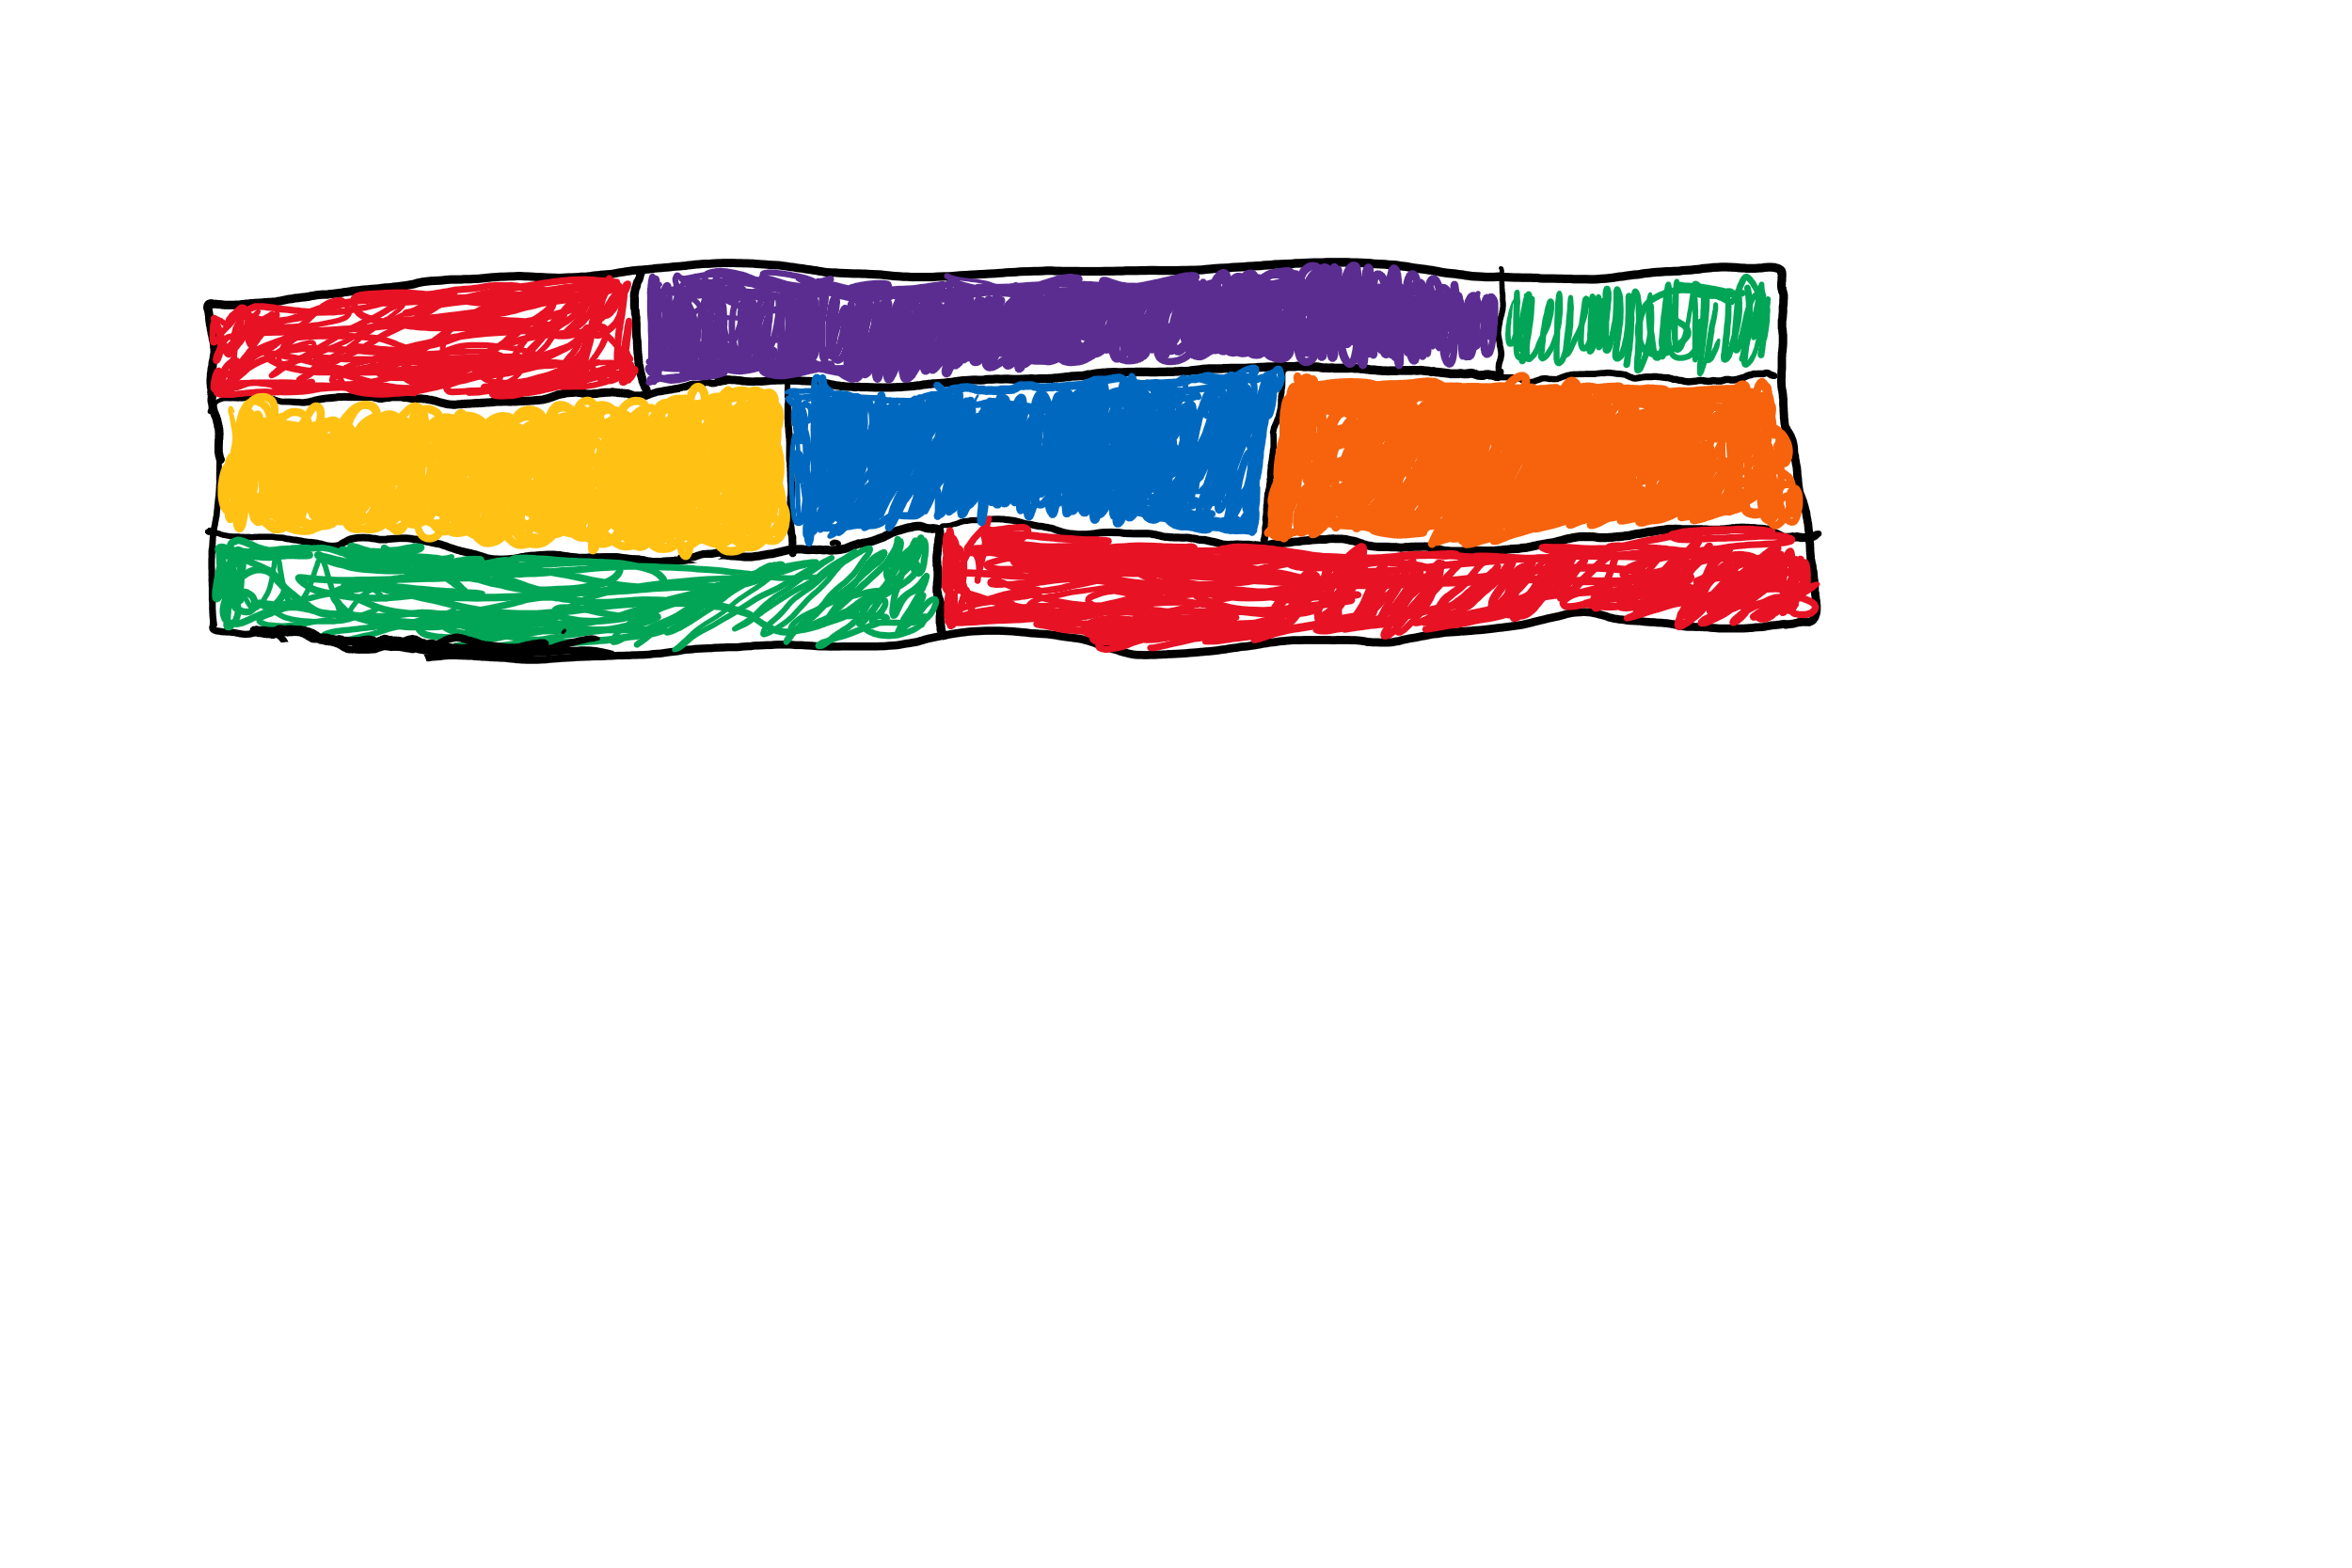
\includegraphics[width=0.75\textwidth]{H-6_4}
		\end{figure}


\end{enumerate}

% ============================================
% ============================================
\collab{n/a}
\nextprob{Shafi Goldwasser}
% ============================================
% ============================================

Write a short (1-2 paragraph) biography of Shafi Goldwasser.
\textbf{In your own words}, describe who they are and why they are important in
the history of computer science.

If you use external resources, please provide
proper citations. If you do not use external sources, please write ``I did not
use any sources to write this biography'' as the last sentence of the
biography.

\paragraph{Answer}

	Shafi Goldwasser is an American born computer scientist who is one of the most acomplished people in the field of cryptography. Born in New York City in 1959, Goldwasser returned to Israel with her family to attend grade school in Tel Aviv. Upon completing high school she returned to the United States where she would obatin her bachleor of science in mathematics from Carnige University, her master's degree and PhD from Berkley both in computer science.

	Soon after recieving her PhD, Goldwasser joined MIT as the first person to hold the title of the RSA proffessorship. Soon after she also joined the Weizmann Institute of Science as a professor. Some of her other achievements and occupations include: member of the theory of computation group at MIT, Director of the Simons Institute for the Theory of Computing at Berkley, and co-recipient of the Turing Award. She has made many contributions to the history of computer science in the area of cryptography and computing theory. Her early work at MIT was reasearch into whether a pseudorandom number generator could be generalized. Her and her team's work on this lead to why we understand why a block cipher can be secure. She also helped define and create what it meant to have an interactive proof and a zero knowledge interactive proof.\footnote{“Shafi Goldwasser.” Shafi Goldwasser - A.M. Turing Award Laureate, \url{amturing.acm.org/award_winners/goldwasser_8627889.cfm}. }\footnote{“Shafi Goldwasser.” Wikipedia, Wikimedia Foundation, 19 Mar. 2021, \url{en.wikipedia.org/wiki/Shafi_Goldwasser}. }

% %% ... the bibliography
% \newpage
% \bibliographystyle{acm}
% \bibliography{biblio}

\end{document}

